\documentclass[11pt,psfig]{article}
\usepackage{epsfig}
\usepackage{times}
\usepackage{amssymb}
\usepackage{float}

\newcount\refno\refno=1
\def\ref{\the\refno \global\advance\refno by 1}
\def\ux{\underline{x}}
\def\uw{\underline{w}}
\def\bw{\underline{w}}
\def\ut{\underline{\theta}}
\def\umu{\underline{\mu}} 
\def\bmu{\underline{\mu}} 
\def\be{p_e^*}
\newcount\eqnumber\eqnumber=1
\def\eq{\the \eqnumber \global\advance\eqnumber by 1}
\def\eqs{\eq}
\def\eqn{\eqno(\eq)}

 \pagestyle{empty}
\def\baselinestretch{1.1}
\topmargin1in \headsep0.3in
\topmargin0in \oddsidemargin0in \textwidth6.5in \textheight8.5in
\begin{document}
\setlength{\parskip}{1.2ex plus0.3ex minus 0.3ex}


\thispagestyle{empty} \pagestyle{myheadings} \markright{Homework
\#: CS 216, Image Understanding: Spring 2014}



\title{CS 216 Homework 2}
\author{Zachary DeStefano, 15247592}
\date{Due Date: April 25, 2014}

\maketitle

\vfill\eject

\newpage

\section*{Problem 1}

We will prove that $(f*g)*h=f*(g*h)$. First off, let $x=f*g$ and let $y=g*h$. \\
\[
x(t) = (f*g)(t) = \sum_{s=-\infty}^{\infty} f(t-s)g(s)
\]
\[
y(t) = (g*h)(t) = \sum_{s=-\infty}^{\infty} g(s)h(t-s)
\]
This means that
\[
(x*h)(t) = \sum_{v=-\infty}^{\infty} x(v)h(t-v) = \sum_{v=-\infty}^{\infty} \sum_{s=-\infty}^{\infty} f(v-s)g(s)h(t-v)
\]
Similarly
\[
(f*y)(t) = \sum_{v=-\infty}^{\infty} f(t-v)y(v) = \sum_{v=-\infty}^{\infty} \sum_{s=-\infty}^{\infty} f(t-v)g(s)h(v-s)
\]
In the second equation, do a change of variables $v = t-v+s$ which does not change the final result since we are going from negative infinity to infinity. For the second equation, we end up with \\
\[
(f*y)(t) = \sum_{v=-\infty}^{\infty} \sum_{s=-\infty}^{\infty} f(v-s)g(s)h(t-v)
\]
This proves that $(x*h)(t)=(f*y)(t)$ and since this applies for any three functions, we have proven that convolution is associative. 

\section*{Problem 2}

If we correlate a function $f$ with an impulse function, then we get $f(-t)$, \\
so the function gets flipped around the y-axis. \\
Here is the proof:\\
Take the impulse function g, so $g(0)=1$ and $g(x)=0$ for all other $x$ \\
Let * be the correlation operation in this case. \\
\[
(f*g)(t) = \sum_{s=-\infty}^{\infty} f(s)g(s+t)
\]
In our case, the inner term is always $0$ except for when $s+t=0$ so $s=-t$, \\
thus $(f*g)(t)=f(-t)$, proving our assertion. \\
\\
Now let $h(t)=g(t)$. We will prove that $(f*g)*h \neq f*(g*h)$. \\
\\
For the right hand side, by what was shown above, \\
$g*h = g$ since the impulse function is symmetric around the y-axis. \\
This means that $f*(g*h)(t) = f*g(t) = f(-t)$. \\
\\
For the left hand side, by what was shown above, \\
$(f*g)(t) = f(-t)$ thus $(f*g)*h(t) = (f(-t))*h(t) = f(t)$\\
\\
For any non-symmetric function $f$, such as $f(t) = 3t+5$, it holds that $f(t) \neq f(-t)$ \\
thus the left hand side is not equal to the right hand side. \\
\\
Since we have example functions whose correlations are not associative, there is no way correlation is associative. 



\section*{Problem 3}

Let $g_1(x) = g_2(y) = N(0,\sigma^2)$. Then
\[
g_1(x) = \frac{1}{\sqrt{2\pi \sigma^2}} e^{-\frac{x^2}{2\sigma^2}}
\]
\[
g_2(y) = \frac{1}{\sqrt{2\pi \sigma^2}} e^{-\frac{y^2}{2\sigma^2}}
\]
This means that
\[
g_1(x)g_2(y) = \frac{1}{2\pi \sigma^2} e^{-\frac{x^2 + y^2}{2\sigma^2}}
\]
This allows us to say that $g(x,y) = g_1(x)g_2(y)$

\section*{Problem 4}

For the spatial domain running time, we can think of convolution as for each pixel in the image, we apply the filter to it. \\
Thus there are $H \cdot W$ iterations of the filter\\
Each filter will take $M \cdot N$ time. \\
Thus the time complexity is $O(MNHW)$\\
\\
If we use FFT, this would be the procedure:\\
1. Convert the signal to frequency\\
2. Convert the filter to frequency \\
3. Do element wise multiplication of the two new vectors. \\
4. Convert the elements back. \\
\\
Step 1 will take $MN \cdot log(MN)$ time\\
Step 2 will take $HW \cdot log(HW)$ time\\
Step 3 will take $max(HW,MN)$ time. The identity of the max will not matter in the end since the previous step eclipses this one. \\
Step 4 will take $max(HW,MN) log( max(HW, MN) )$ time. Again which one is the max does not matter because of step 1 and 2. \\
\\
The total running time is thus $O(MN \cdot log(MN) + HW \cdot log(HW) )$ time. \\
Assuming that $HW$ is the max, the running time is $O(HW \cdot log(HW))$. \\
\\
If the filter is $f(x,y) = f(x)g(y)$ then we could do the following:\\
1. Compute the horizontal filter\\
2. Compute the vertical filter\\
3. Do point wise multiplication \\
\\
Step 1 will take $HWM$ time and step 2 will be $HWN$ time. \\
Step 3 will be $HW$ time. \\
Total running time is thus $O( HW(M+N) )$ time. \\
TODO: Improve the algorithm and its analysis for the case of a filter being that product. 

\section*{Problem 5}

Our two gaussians are as follows
\[
g_1(t) = \frac{1}{\sqrt{2\pi \sigma_1^2}} e^{-\frac{t^2}{2\sigma_1^2}}
\]
\[
g_2(t) = \frac{1}{\sqrt{2\pi \sigma_2^2}} e^{-\frac{t^2}{2\sigma_2^2}}
\]
The convolution formula we will use is the following
\[
g_3(t) = \int_{-\infty}^{\infty}{g_1(s)g_2(t-s) \, ds}
\]
\\
Page 6 of this paper has a good explanation
\begin{verbatim}
http://www.tina-vision.net/docs/memos/2003-003.pdf
\end{verbatim}
Let $F_1$ be the Fourier transform for $g_1$ and $F_2$ be the transform for $g_2$.\\
\[
F_1(t) = \int_{-\infty}^{\infty}{g_1(s) e^{-2\pi i s t} \, ds}
\]
\[
F_2(t) = \int_{-\infty}^{\infty}{g_2(s) e^{-2\pi i s t} \, ds}
\]
Expanding we have
\[
F_1(t) = \frac{1}{\sqrt{2 \pi \sigma_1^2}} \int_{-\infty}^{\infty}{e^{-\frac{s^2}{2\sigma_1^2}} e^{-2\pi i s t} \, ds}
\]
\[
F_1(t) = \frac{1}{\sqrt{2 \pi \sigma_2^2}} \int_{-\infty}^{\infty}{e^{-\frac{s^2}{2\sigma_2^2}} e^{-2\pi i s t} \, ds}
\]

\section*{Problem 6}

Here are the initial plots

\begin{figure}[H]
\centering
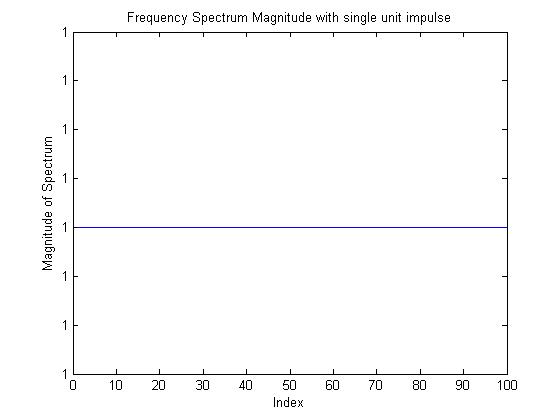
\includegraphics[height=3in]{prob6plot_freq1.jpg}
\caption{Frequency Spectrum Magnitude Plot for single impulse}
\end{figure}

\begin{figure}[H]
\centering
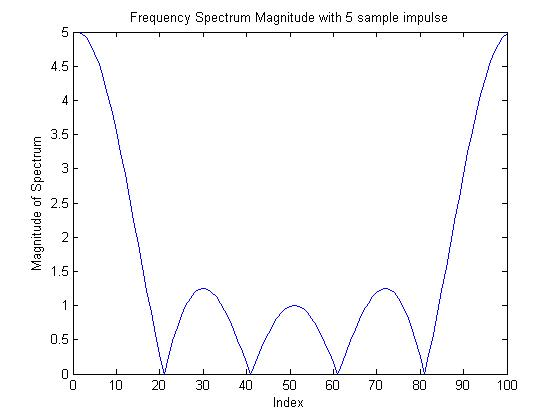
\includegraphics[height=3in]{prob6plot_freq5.jpg}
\caption{Frequency Spectrum Magnitude Plot for 5 sample impulse}
\end{figure}

\begin{figure}[H]
\centering
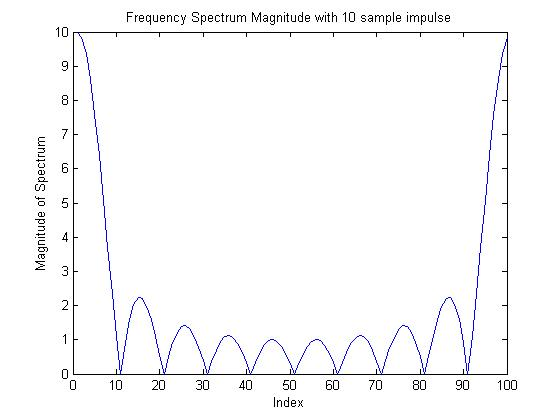
\includegraphics[height=3in]{prob6plot_freq10.jpg}
\caption{Frequency Spectrum Magnitude Plot for 10 sample impulse}
\end{figure}

\begin{figure}[H]
\centering
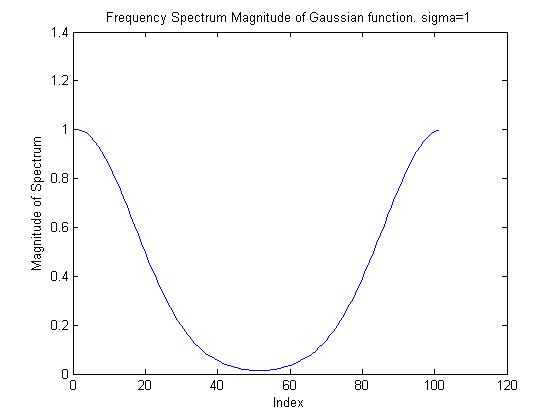
\includegraphics[height=3in]{prob6plot_freqGauss1.jpg}
\caption{Frequency Spectrum Magnitude Plot for Gaussian Function with $\sigma=1$}
\end{figure}

\begin{figure}[H]
\centering
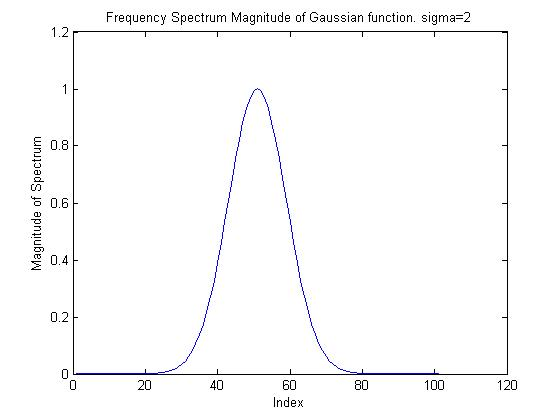
\includegraphics[height=3in]{prob6plot_freqGauss2.jpg}
\caption{Frequency Spectrum Magnitude Plot for Gaussian Function with $\sigma=2$}
\end{figure}

Here is the magnitude, phase experiment results

\begin{figure}[H]
\centering
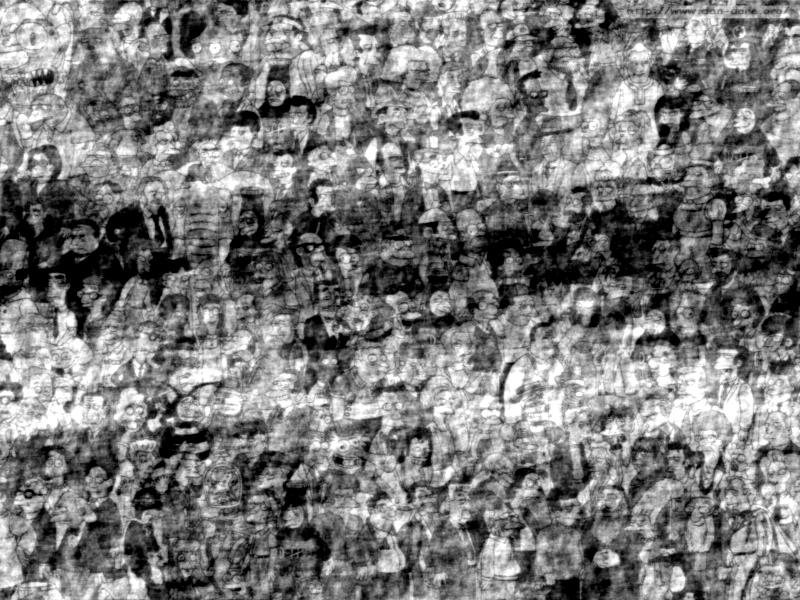
\includegraphics[height=3in]{mag_zebra_phase_simpsons.jpg}
\caption{Magnitude of Zebra picture with Phase of Simpsons picture}
\end{figure}

\section*{Problem 7}

Pictures for the Zebra image

\begin{figure}[H]
\centering
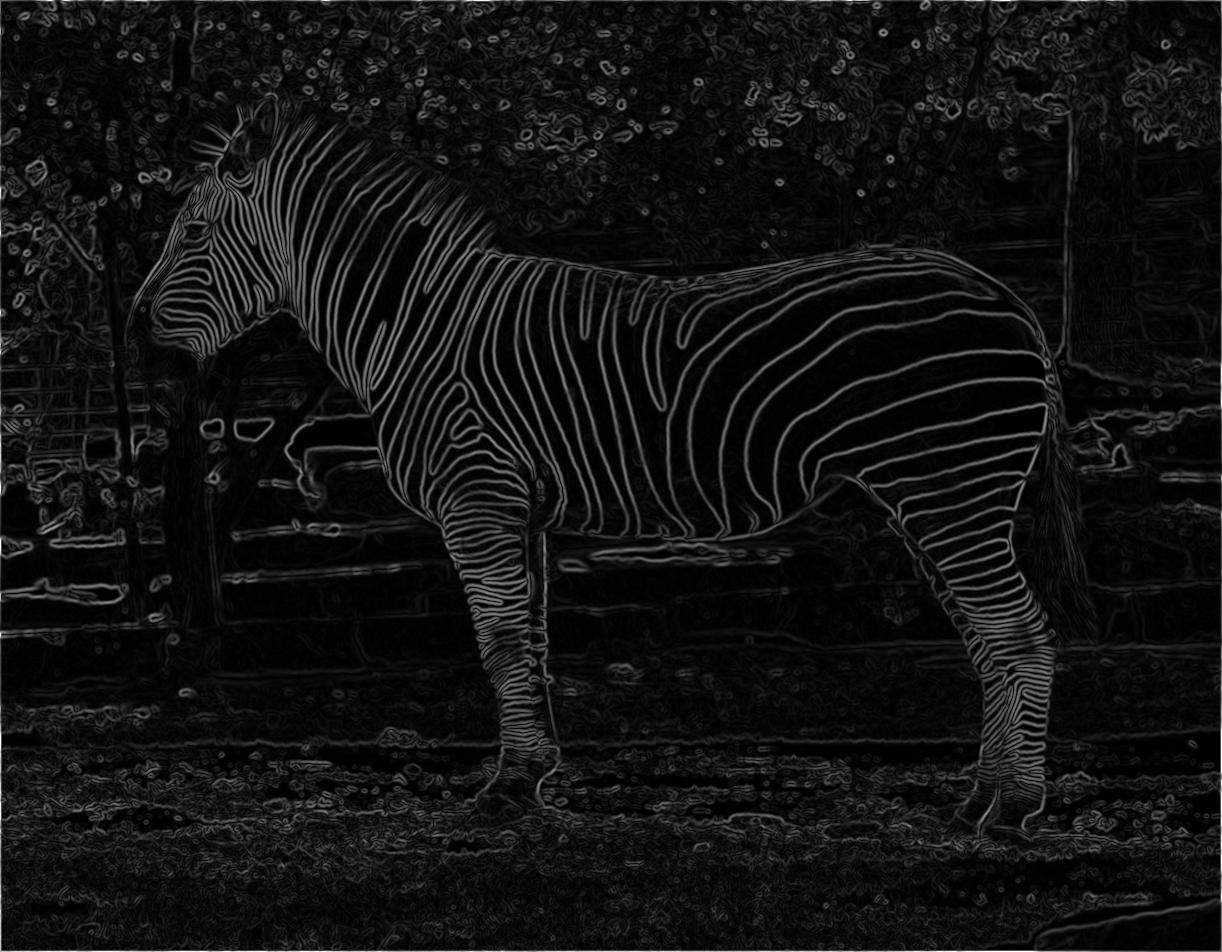
\includegraphics[height=3in]{magGradient_zebra1.jpg}
\caption{Magnitude of the Gradient of the zebra picture where $\sigma=3$}
\end{figure}

\begin{figure}[H]
\centering
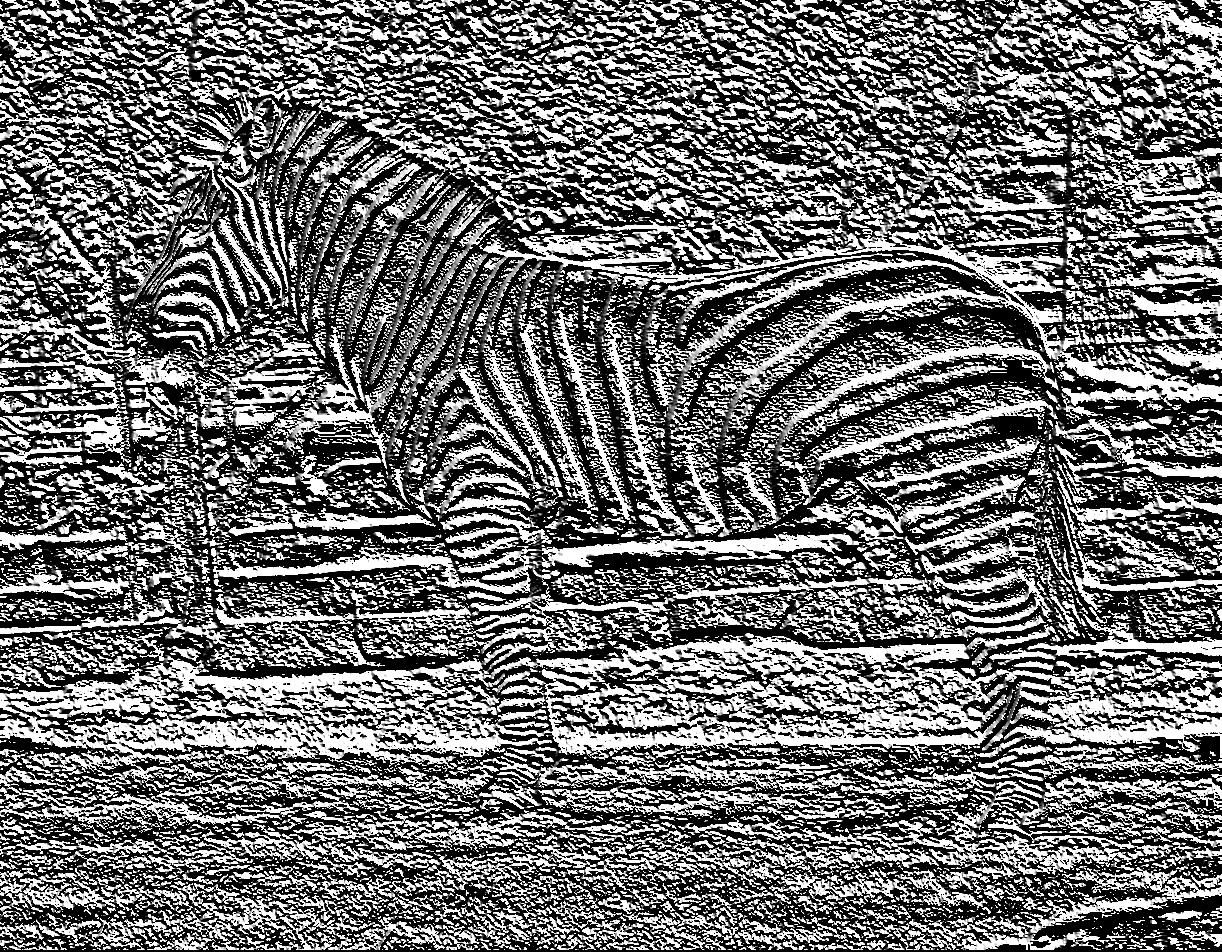
\includegraphics[height=3in]{orientGradient_zebra1.jpg}
\caption{Orientation of the Gradient of the zebra picture where $\sigma=3$}
\end{figure}

With new sigma

\begin{figure}[H]
\centering
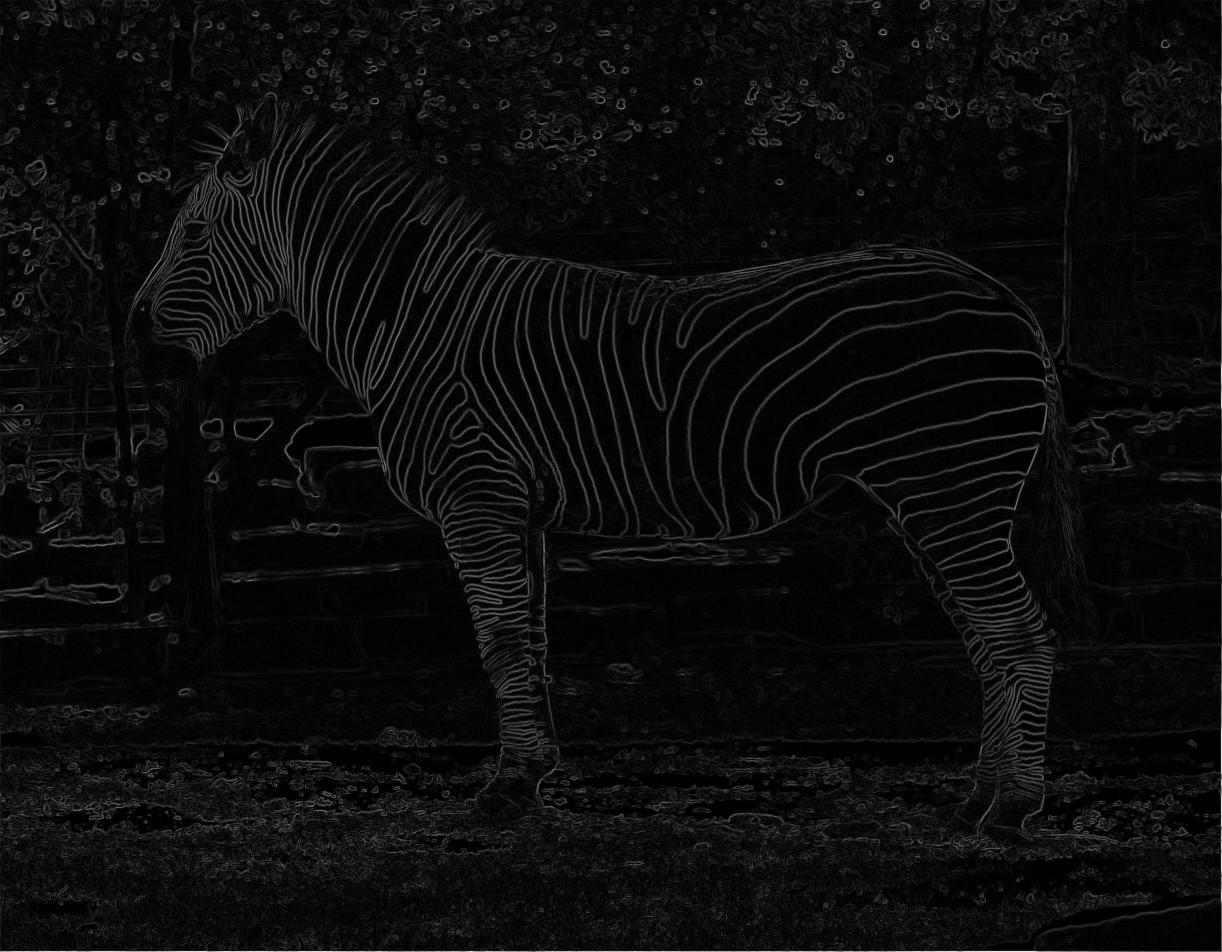
\includegraphics[height=3in]{magGradient2_zebra1.jpg}
\caption{Magnitude of the Gradient of the zebra picture where $\sigma=2$}
\end{figure}

\begin{figure}[H]
\centering
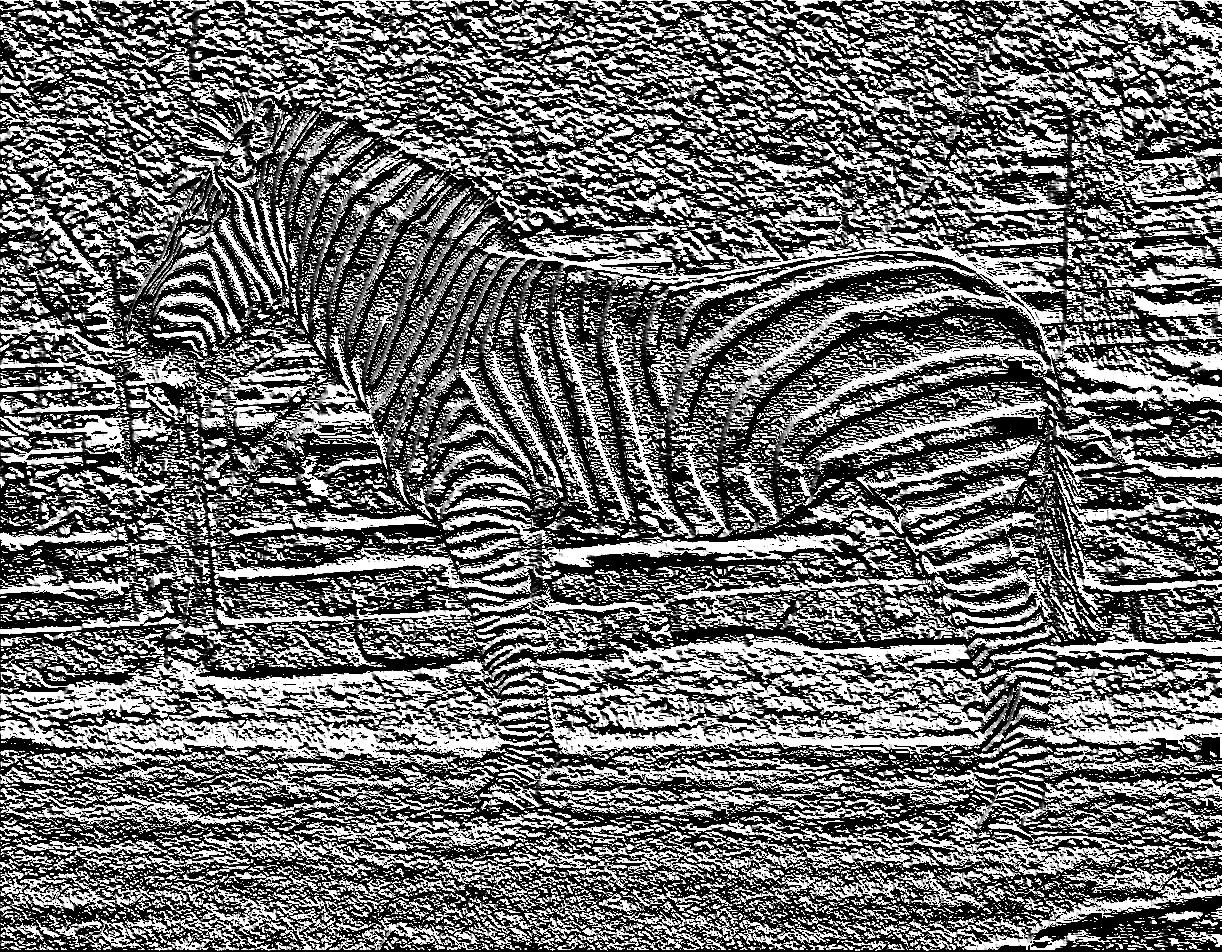
\includegraphics[height=3in]{orientGradient2_zebra1.jpg}
\caption{Orientation of the Gradient of the zebra picture where $\sigma=2$}
\end{figure}

\end{document}








